\documentclass[final]{siamltexmm}
\documentclass[10pt,a4paper]{article}

\usepackage{graphicx}
\usepackage{algorithm}
\usepackage{algorithmic}

% \usepackage[demo]{graphicx}
% \usepackage{subfig}

\newcommand{\pe}{\psi}
\def\d{\delta} 
\def\ds{\displaystyle} 
\def\e{{\epsilon}} 
\def\eb{\bar{\eta}}  
\def\enorm#1{\|#1\|_2} 
\def\Fp{F^\prime}  
\def\fishpack{{FISHPACK}} 
\def\fortran{{FORTRAN}} 
\def\gmres{{GMRES}} 
\def\gmresm{{\rm GMRES($m$)}} 
\def\Kc{{\cal K}} 
\def\norm#1{\|#1\|} 
\def\wb{{\bar w}} 
\def\zb{{\bar z}} 

% some definitions of bold math italics to make typing easier.
% They are used in the corollary.

\def\bfE{\mbox{\boldmath$E$}}
\def\bfG{\mbox{\boldmath$G$}}

\title{Deep Learning Assignment 2}
\author{Yun-shao Sung\thanks{\tt yss265@nyu.edu}
        \and Chung-Ling Yao\thanks{\tt cly264@nyu.edu}}

\begin{document}
\maketitle

\begin{abstract}
This is the report for deep learning assignment 2
\end{abstract}

\pagestyle{myheadings}
\thispagestyle{plain}

\section{More Backpropagation}
\subsection{Backpropagation through a DAG of modules}
Given each node is sigmoid layers, and the second layer is $O_{min} = min(i_{1}, i_{2})$ and $O_{max} = max(i_{1}, i_{2})$. Therefore, we can rewrite $y$ as:
\begin{equation}
y = min({1\over1+e^{-x_{1}}}, {1\over1+e^{-x_{2}}}) + max({1\over1+e^{-x_{1}}}, {1\over1+e^{-x_{2}}})
\end{equation}
which can also rewrite as:
\begin{equation}
y = {1\over1+e^{-x_{1}}} + {1\over1+e^{-x_{2}}}
\end{equation}
as we taking the deritive of $E$ respect to $x_{i}$ and with chain rule applied:
\begin{equation}
{\partial E\over \partial x_{i}} = {\partial E\over \partial y} {e^{-x_{i}} \over (1+e^{x_{i}})^2}}
\end{equation}

\subsection{Batch Normalization}

\\
\section{STL-10: semi-supervised image recognition}
\subsection{Method: Surrogate Class}
\subsection{Method: K­means Centroids}
Hi
\begin{figure}[H]
\centering
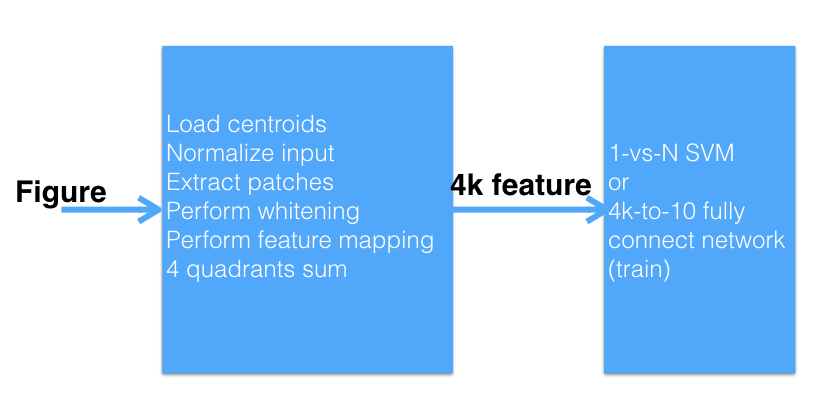
\includegraphics[width=100mm]{../fig/kmeans.png}
  \caption{Kmeans model}
\end{figure}

\subsection{Method: Pseudo­labels}
Hi
\begin{figure}[H]
\centering
\includegraphics[width=100mm]{../fig/Pseudo­labels.png}
  \caption{Pseudo­labels model}
\end{figure}

\subsection{Method: K­means Centroids + Pseudo­labels}



\\
\section{Visualization}
\subsection{Visualizing filters and augmentations}
Initially we were also trying to creat surrogate data set from 4000 unlabel figures, each figure will produced 100 surrogate figures and therefore we got 4000 class of 400000 figures in total. The initial figre is in the size of 3x96x96, and we created the surrogate figure by the size of 3x32x32 and each will subject in a random degree of rotation between -20 to 20, vertical and horizontal translate between 0 to 0.1, and scale in the range between 0.7 to 1.4. Figure 3.1 is the visualization of the surrogate figures.
\begin{figure}[H]
\centering
\begin{subfigure}
  \begin{tabular}{c}
  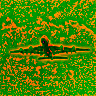
\includegraphics[width=50mm]{../fig/img_regNorm/2.png}
  \end{tabular}{}
\end{subfigure}
\begin{subfigure}
  \begin{tabular}{cccc}
  \subfloat{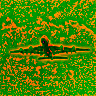
\includegraphics[width = 10mm]{../fig/img_regNorm/2.png}}&
  \subfloat{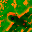
\includegraphics[width = 10mm]{../fig/img/2_1.png}}&
  \subfloat{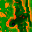
\includegraphics[width = 10mm]{../fig/img/2_2.png}}&
  \subfloat{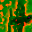
\includegraphics[width = 10mm]{../fig/img/2_19.png}}\\
  \subfloat{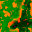
\includegraphics[width = 10mm]{../fig/img/2_3.png}}&
  \subfloat{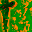
\includegraphics[width = 10mm]{../fig/img/2_4.png}}&
  \subfloat{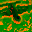
\includegraphics[width = 10mm]{../fig/img/2_5.png}}&
  \subfloat{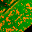
\includegraphics[width = 10mm]{../fig/img/2_10.png}}\\
  \subfloat{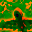
\includegraphics[width = 10mm]{../fig/img/2_25.png}}&
  \subfloat{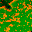
\includegraphics[width = 10mm]{../fig/img/2_26.png}}&
  \subfloat{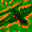
\includegraphics[width = 10mm]{../fig/img/2_29.png}}&
  \subfloat{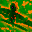
\includegraphics[width = 10mm]{../fig/img/2_30.png}}\\
  \subfloat{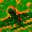
\includegraphics[width = 10mm]{../fig/img/2_32.png}}&
  \subfloat{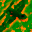
\includegraphics[width = 10mm]{../fig/img/2_33.png}}&
  \subfloat{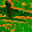
\includegraphics[width = 10mm]{../fig/img/2_34.png}}&
  \subfloat{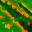
\includegraphics[width = 10mm]{../fig/img/2_35.png}}\\
  \subfloat{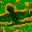
\includegraphics[width = 10mm]{../fig/img/2_37.png}}&
  \subfloat{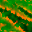
\includegraphics[width = 10mm]{../fig/img/2_38.png}}&
  \subfloat{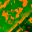
\includegraphics[width = 10mm]{../fig/img/2_41.png}}&
  \subfloat{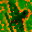
\includegraphics[width = 10mm]{../fig/img/2_48.png}}&
  \end{tabular}
\end{subfigure}
\caption{Figures of surrogate set}
\end{figure}
Then we implemented the kmeans method. According to the paper, they randomly extracted patches from unlabeled set of data, and performed kmean to find the centroids. The size of patch we extracted is 22x22 and we extracted 16 patches from total of 20000 unlabel figures. Number of centroids we obtained is 1600 because it produced good accuracy as the paper mentioned. As we can see from figure 3.2, most of the centroids are in very sharp of edge and color blobs.
\begin{figure}[H]
\centering
\begin{subfigure}
  \begin{tabular}{c}
  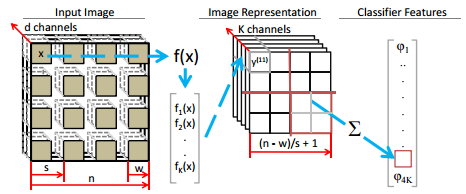
\includegraphics[width=100mm]{../fig/kmeansMethod.png}
  \end{tabular}{}
\end{subfigure}
\begin{subfigure}
  \begin{tabular}{cccc}
  \subfloat{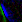
\includegraphics[width = 10mm]{../fig/center_20000_700/center4.png}}&
  \subfloat{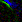
\includegraphics[width = 10mm]{../fig/center_20000_700/center5.png}}&
  \subfloat{
\includegraphics[width = 10mm]{../fig/center_20000_700/center6.png}}&
  \subfloat{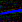
\includegraphics[width = 10mm]{../fig/center_20000_700/center8.png}}\\
  \subfloat{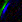
\includegraphics[width = 10mm]{../fig/center_20000_700/center12.png}}&
  \subfloat{
\includegraphics[width = 10mm]{../fig/center_20000_700/center22.png}}&
  \subfloat{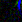
\includegraphics[width = 10mm]{../fig/center_20000_700/center23.png}}&
  \subfloat{
\includegraphics[width = 10mm]{../fig/center_20000_700/center24.png}}\\
  \subfloat{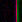
\includegraphics[width = 10mm]{../fig/center_20000_700/center28.png}}&
  \subfloat{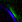
\includegraphics[width = 10mm]{../fig/center_20000_700/center30.png}}&
  \subfloat{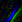
\includegraphics[width = 10mm]{../fig/center_20000_700/center36.png}}&
  \subfloat{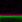
\includegraphics[width = 10mm]{../fig/center_20000_700/center37.png}}\\
  \subfloat{
\includegraphics[width = 10mm]{../fig/center_20000_700/center38.png}}&
  \subfloat{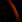
\includegraphics[width = 10mm]{../fig/center_20000_700/center41.png}}&
  \subfloat{
\includegraphics[width = 10mm]{../fig/center_20000_700/center46.png}}&
  \subfloat{
\includegraphics[width = 10mm]{../fig/center_20000_700/center49.png}}\\
  \subfloat{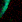
\includegraphics[width = 10mm]{../fig/center_20000_700/center50.png}}&
  \subfloat{
\includegraphics[width = 10mm]{../fig/center_20000_700/center52.png}}&
  \subfloat{
\includegraphics[width = 10mm]{../fig/center_20000_700/center57.png}}&
  \subfloat{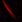
\includegraphics[width = 10mm]{../fig/center_20000_700/center58.png}}&
  \end{tabular}
\end{subfigure}
\caption{Figure of centroids}
\end{figure}

\subsection{t-SNE}
Here we took all the images from val.t7b, which contains 1000 figures for total and 100 figures in each of class. To generate t-SNE embedding, we used only the first channel of each of the image, which the dimension is 1x96x96, and feed it into manifold.embedding.tsne. Then we will get the mapping result for each of the image onto the 2D space, and we can plot the figures based on the mapped coordinate.

\begin{figure}[H]
  \centering
    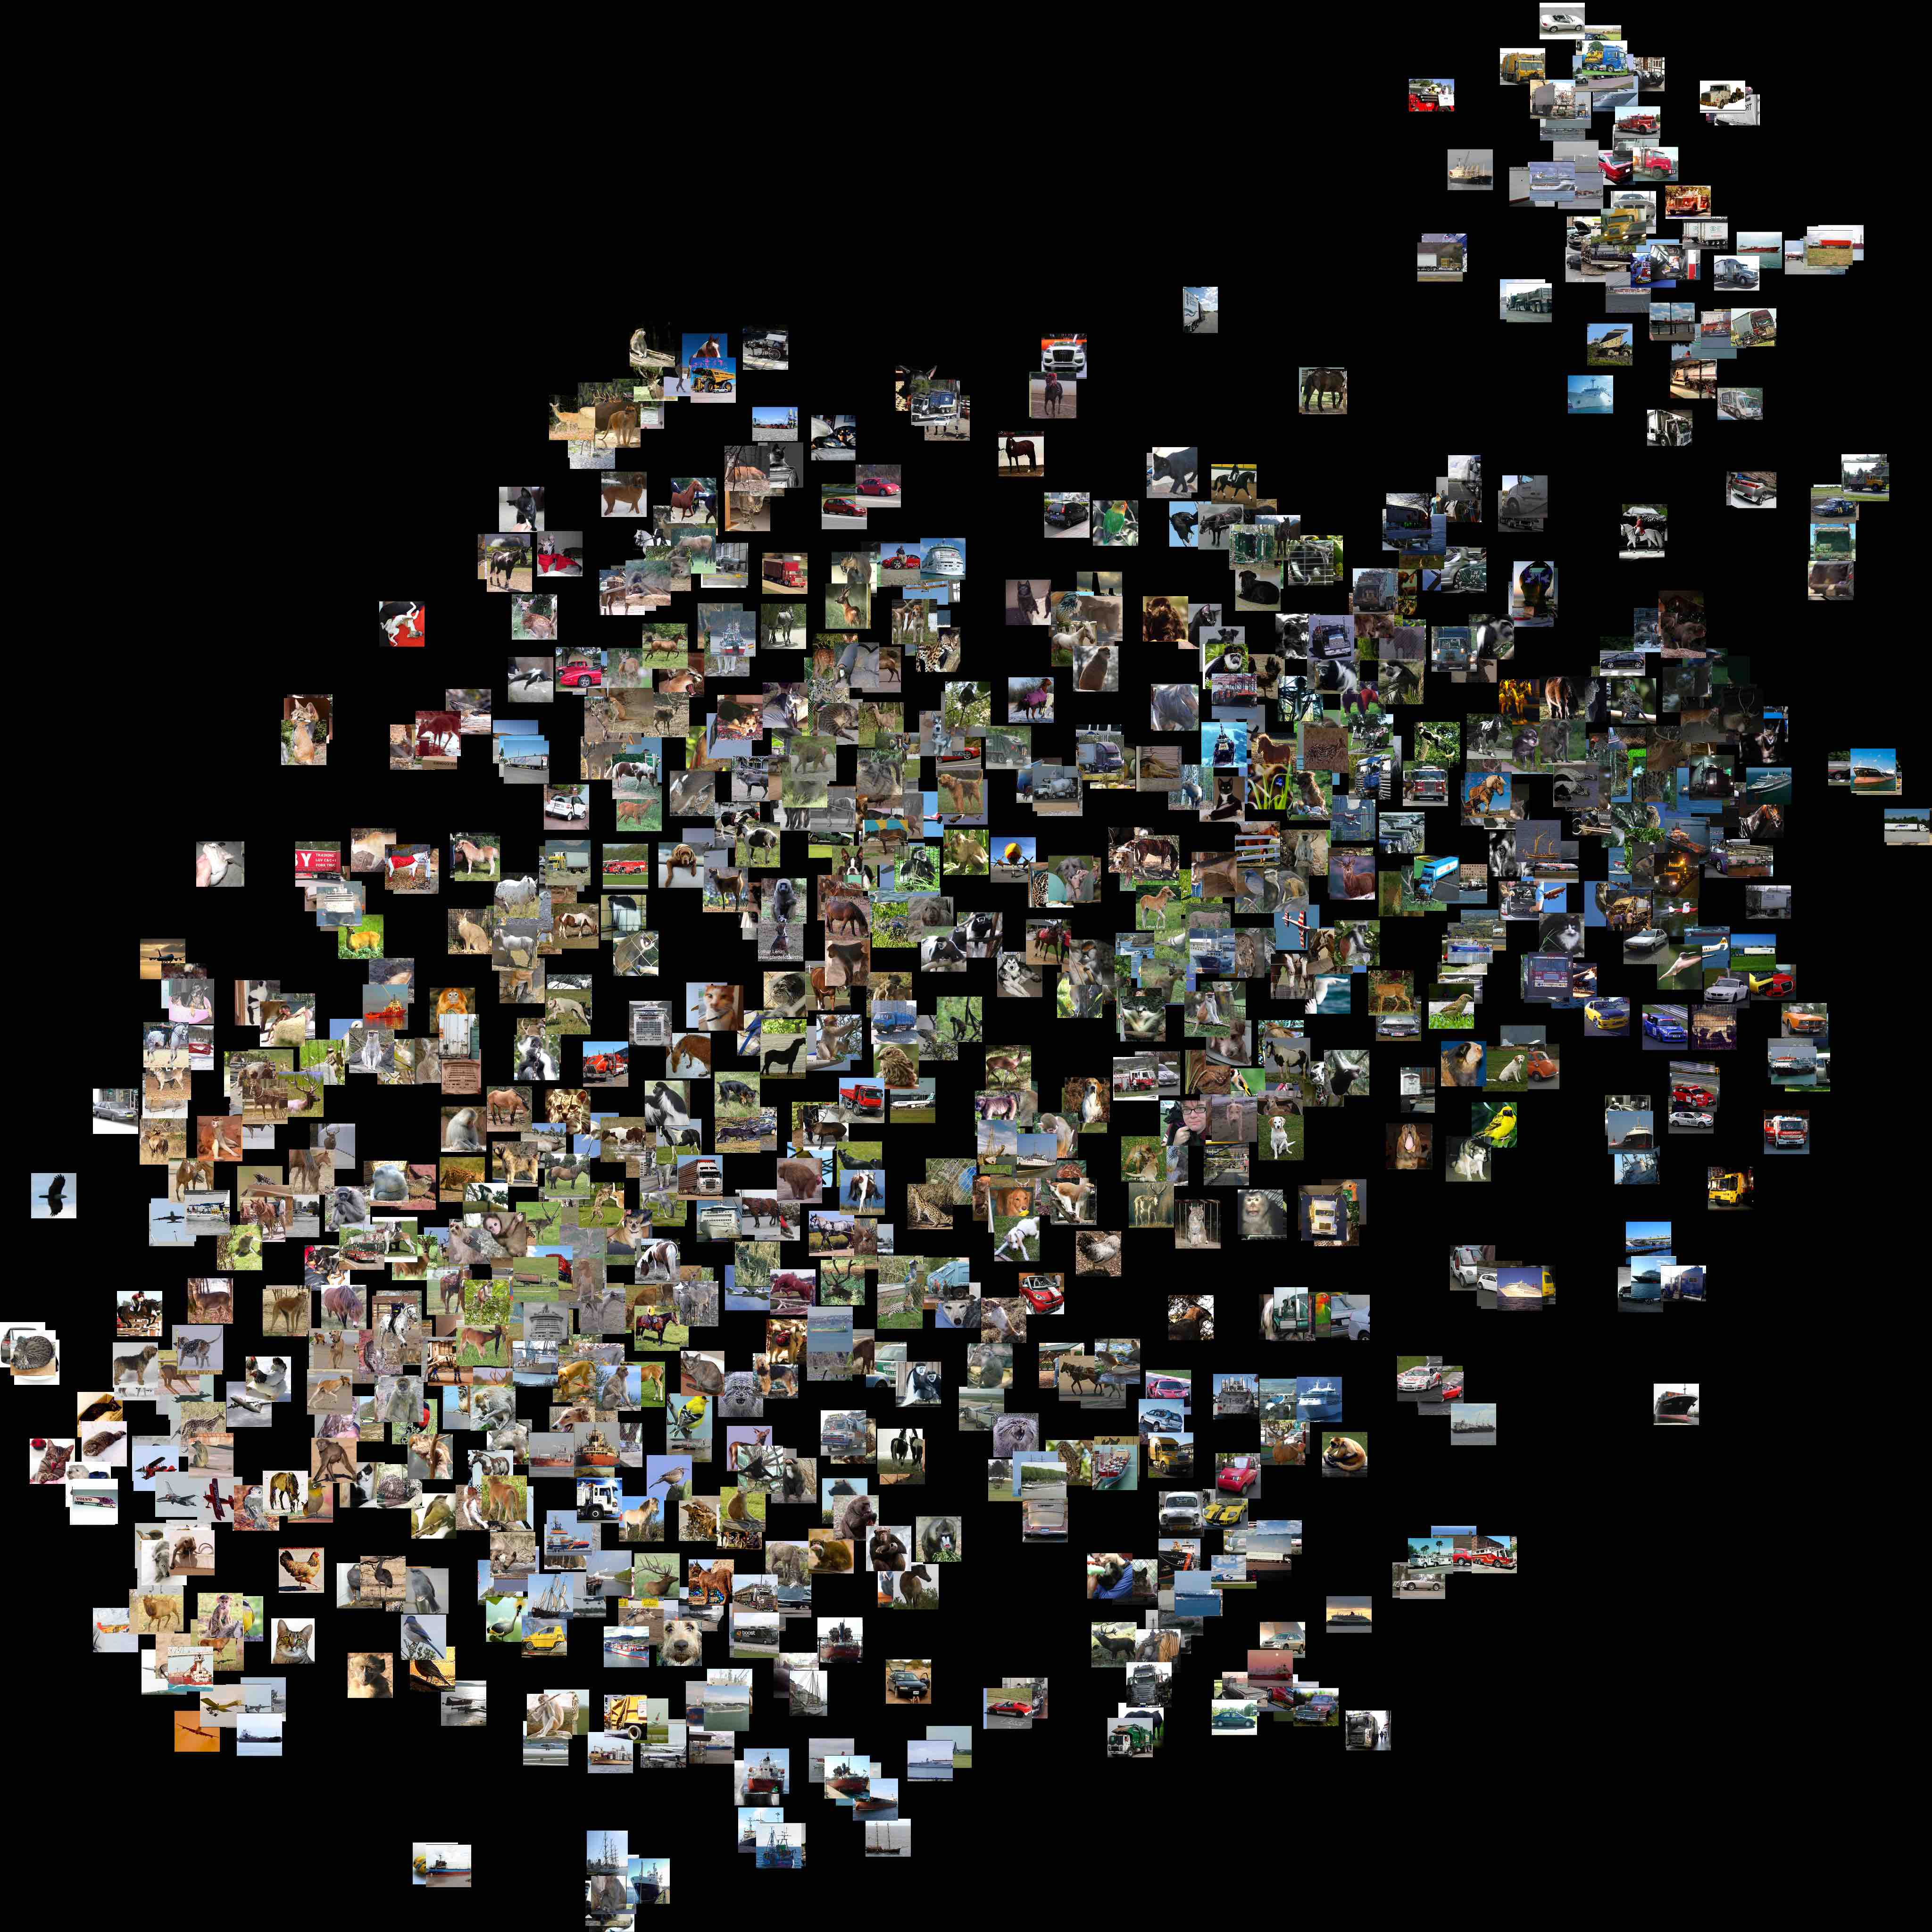
\includegraphics[width=100mm]{../fig/t_SNEIII.jpeg}
  \caption{The training and test accuracy of 3-layer versus 2-layer model}
\end{figure}

\end{document}

